\documentclass{article}

\usepackage{blindtext}
\usepackage{titlesec}
\usepackage{polski}
\usepackage[utf8]{inputenc}
\usepackage[T1]{fontenc}
\usepackage[polish]{babel}
\usepackage{graphicx}

\graphicspath{ {./photos/} }
\begin{document}

\title{Fishing Forum Dokumentacja}
\author{
  Wojciech Pietruszewski - 275023 \\
  Adam Pilarski - 275020 \\
  Szymon Merski - 274979}
\date{\today}

\maketitle
\newpage
\tableofcontents

\newpage
\section{Wstęp}
Aplikacja 'Fishing Forum' to interaktywna przestrzeń online, stworzona z myślą o wspólnym dzieleniu się wiedzą, poradami, a takze o umożliwieniu nawiązania nowych znajomości. Użytkownicy mogą tworzyć wątki, w których inni użytkownicy mogą komentować, a także oceniać. Każdy użytkownik ma możliwość stworzenia własnego profilu, na którym może umieścić zdjęcie, opis, a także informacje o swoich ulubionych wędkarskich miejscach.

\section{Technologie i biblioteki}
W tworzeniu aplikacji wykorzystaliśmy:
\subsection{Backend}
\begin{itemize}
  \item Node.js 26.0
  \item Express.js 4.18.1
  \item BcryptJs 2.4.3
  \item Cors 2.8.5
  \item Dotenv 16.3.1
  \item Jsonwebtoken 9.0.2
  \item Mongoose 8.0.4
  \item Morgan 1.10.0
  \item Ws 8.16.0
  \item Zod 3.22.4
\end{itemize}
\subsection{Frontend}
\begin{itemize}
  \item React 18.2.0
  \item React-dom 18.2.0
  \item React-router-dom 6.21.2
  \item React-icons 5.0.1
  \item React-leaflet 4.2.1
  \item Axios 1.6.5
  \item Tailwindcss 3.4.1
  \item Eslint 8.55.0
  \item Vite 5.0.8
  \item Typescript 5.2.2
\end{itemize}
\subsection{Baza danych}
\begin{itemize}
  \item MongoDB
\end{itemize}
\section{Model bazy danych}
Do stworzenia bazy danych wykorzystaliśmy MongoDB. Ta nierelacyjna baza danych pozwala na przechowywanie danych w postaci dokumentów, które są zapisywane w formacie JSON. W bazie danych przechowujemy informacje o użytkownikach, wątkach, komentarzach, a także o miejscach wędkarskich. Poniżej przedstawiamy pełny spis kolekcji wraz z ich polami.
\subsection{Kolekcja użytkowników}
\begin{itemize}
  \item \_id - identyfikator użytkownika
  \item username - nazwa użytkownika
  \item dateOfRegistration - data rejestracji użytkownika
  \item description - opis użytkownika
  \item profilePicture - zdjęcie profilowe użytkownika
  \item location - lokalizacja użytkownika
  \item score - liczba punktów użytkownika
  \item rank - ranga użytkownika
  \item password - hasło użytkownika
  \item posts - tablica identyfikatorów wątków użytkownika
  \item badges - tablica identyfikatorów odznak użytkownika
  \item conversations - tablica identyfikatorów konwersacji użytkownika
  \item friends - tablica identyfikatorów znajomych użytkownika
  \item fishingSpots - tablica identyfikatorów miejsc wędkarskich użytkownika
\end{itemize}
\subsection{Kolekcja miejsc wędkarskich}
\begin{itemize}
  \item \_id - identyfikator miejsca wędkarskiego
  \item name - nazwa miejsca wędkarskiego
  \item longitude - długość geograficzna miejsca wędkarskiego
  \item latitude - szerokość geograficzna miejsca wędkarskiego
  \item description - opis miejsca wędkarskiego
  \item rating - ocena miejsca wędkarskiego
  \item type - typ miejsca wędkarskiego
  \item image - zdjęcie miejsca wędkarskiego
  \item author - identyfikator autora miejsca wędkarskiego
\end{itemize}
\subsection{Kolekcja wątków}
\begin{itemize}
  \item \_id - identyfikator wątku
  \item name - nazwa wątku
  \item description - opis wątku
  \item numberOfPosts - liczba postów w wątku
  \item lastPost - identyfikator ostatniego postu w wątku
\end{itemize}
\subsection{Kolekcja postów}
\begin{itemize}
  \item \_id - identyfikator postu
  \item title - tytuł postu
  \item content - treść postu
  \item creationDate - data utworzenia postu
  \item type - typ postu
  \item lastResponse - identyfikator ostatniej odpowiedzi w wątku
  \item topic - identyfikator wątku, do którego należy post
  \item author - identyfikator autora postu
  \item responses - tablica identyfikatorów odpowiedzi na post
\end{itemize}
\subsection{Kolekcja odpowiedzi}
\begin{itemize}
  \item \_id - identyfikator odpowiedzi
  \item content - treść odpowiedzi
  \item creationDate - data utworzenia odpowiedzi
  \item post - identyfikator postu, do którego należy odpowiedź
  \item author - identyfikator autora odpowiedzi
\end{itemize}
\subsection{Kolekcja odznak}
\begin{itemize}
  \item \_id - identyfikator odznaki
  \item name - nazwa odznaki
  \item icon - ikona odznaki
\end{itemize}
\subsection{Kolekcja konwersacji}
\begin{itemize}
  \item \_id - identyfikator konwersacji
  \item members - tablica identyfikatorów uczestników konwersacji
  \item messages - tablica identyfikatorów wiadomości w konwersacji
\end{itemize}
\subsection{Kolekcja wiadomości}
\begin{itemize}
  \item \_id - identyfikator wiadomości
  \item content - treść wiadomości
  \item date - data utworzenia wiadomości
  \item isRead - informacja o tym, czy wiadomość została przeczytana
  \item sender - identyfikator nadawcy wiadomości
\end{itemize}
\subsection{Kolekcja ticketów}
\begin{itemize}
  \item \_id - identyfikator ticketu
  \item email - adres email osoby, która wysłała ticket
  \item content - treść ticketu
  \item creationDate - data utworzenia ticketu
\end{itemize}
\section{Funckje}

\subsection{Dla niezalogowanych użytkowników}
\subsubsection{Przeglądanie wątków}
\frame{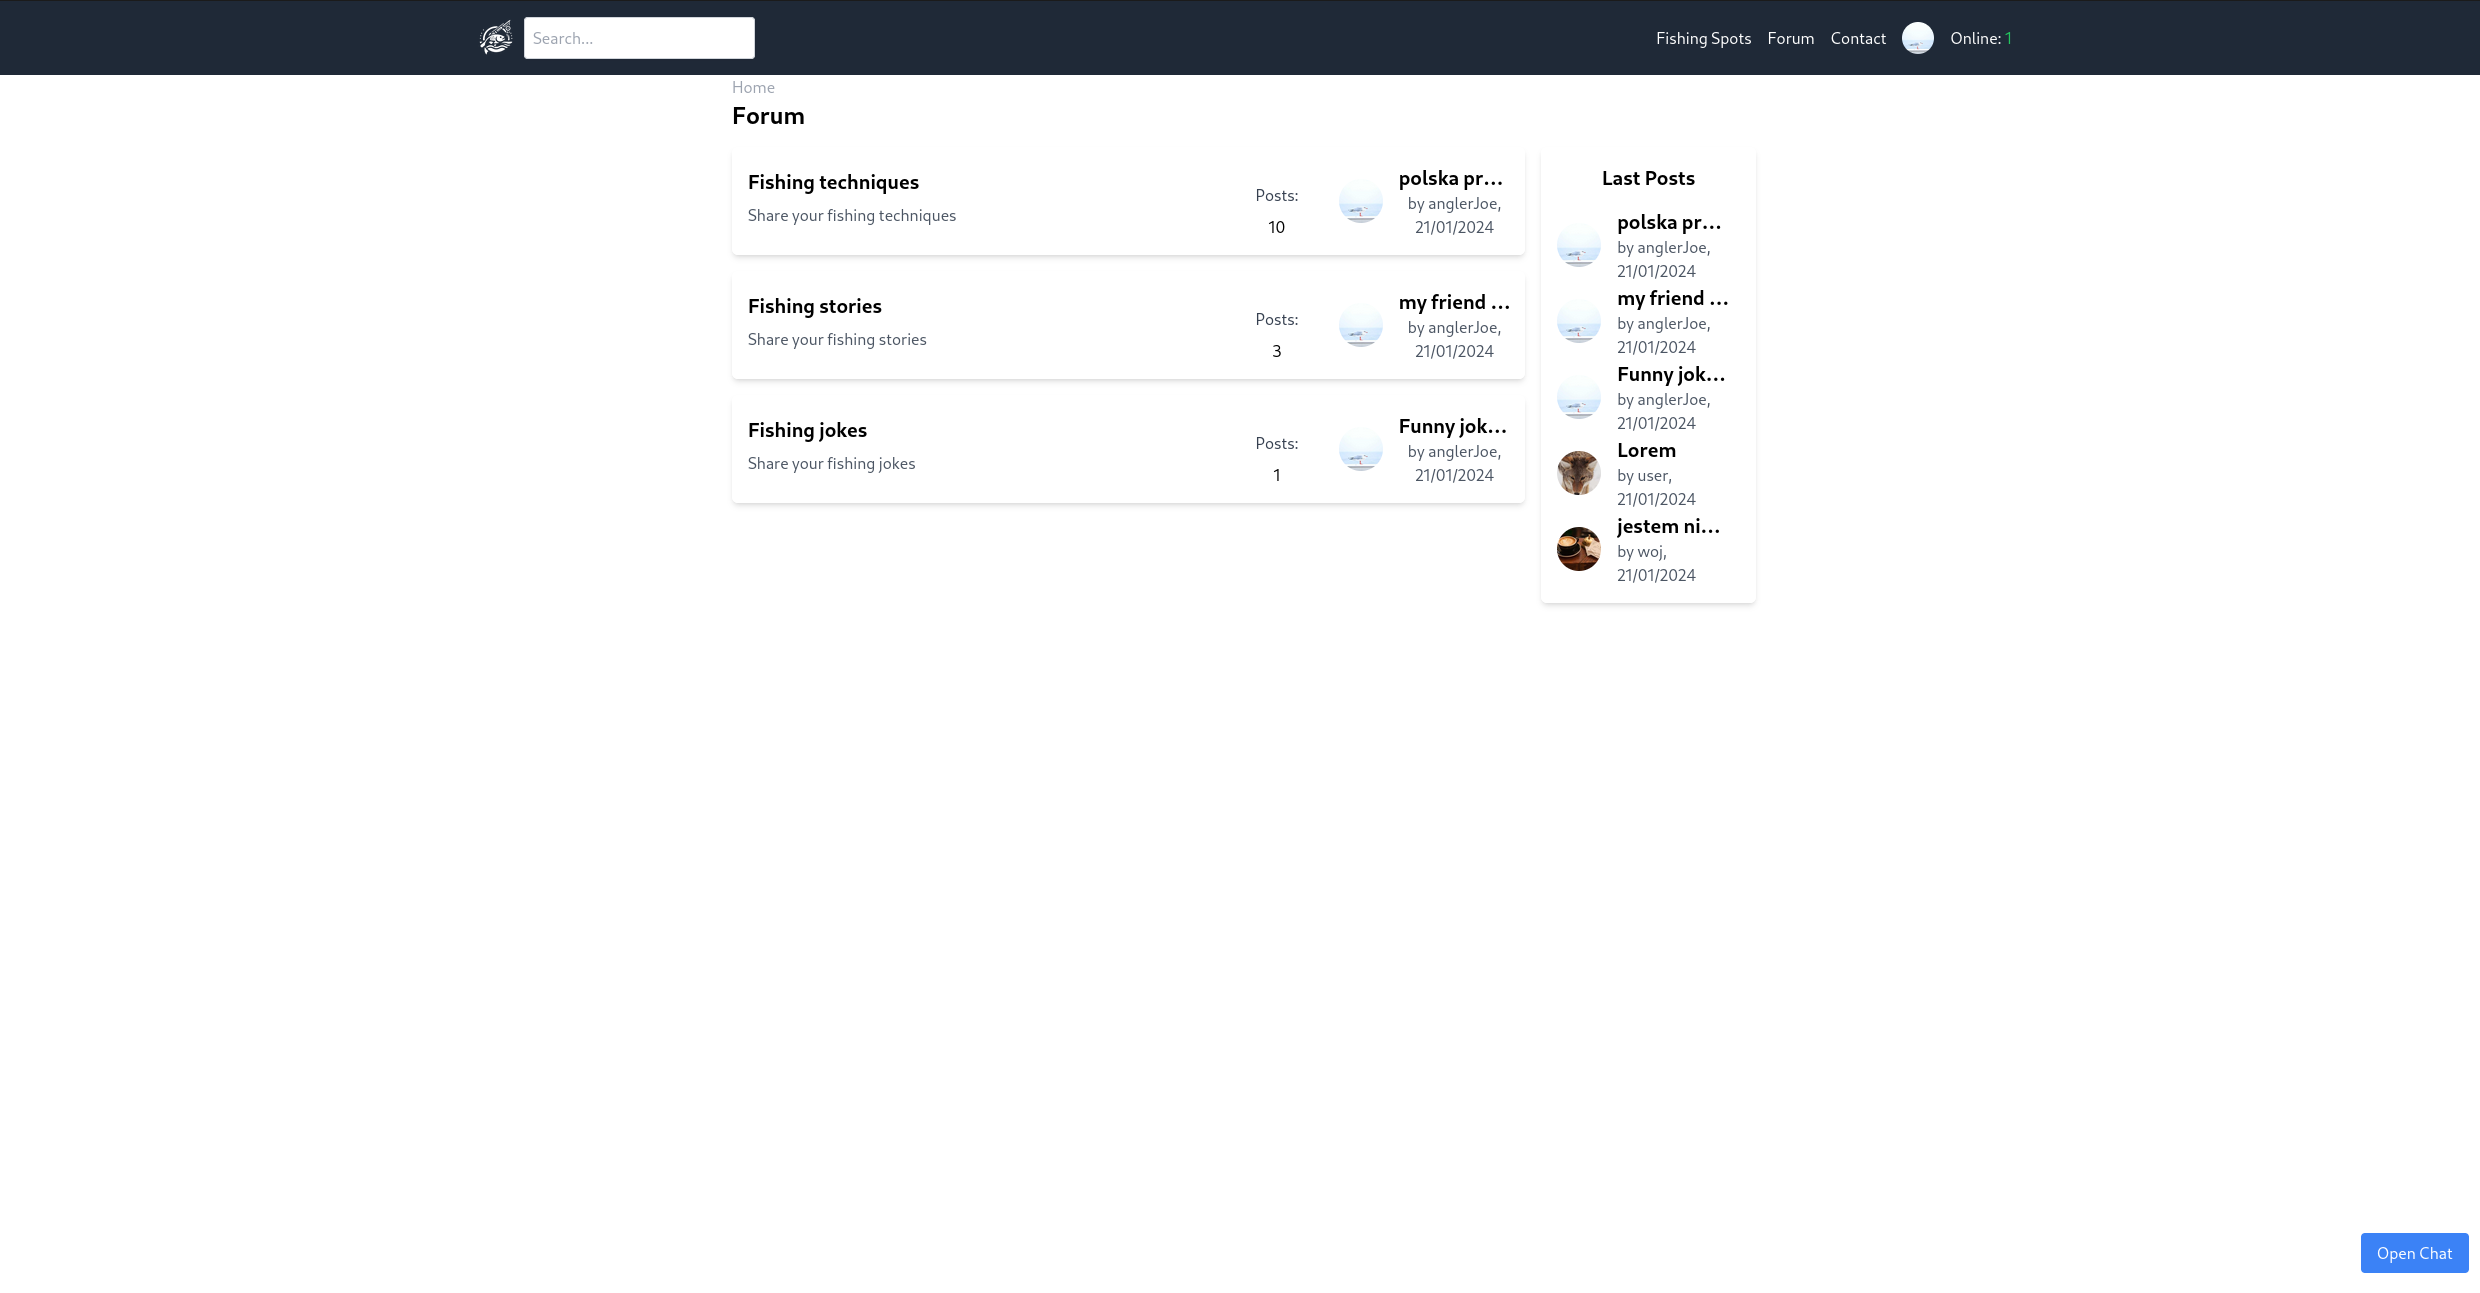
\includegraphics[width=\textwidth]{forum_topics.png}}
\subsubsection{Przeglądanie miejsc wędkarskich}
\frame{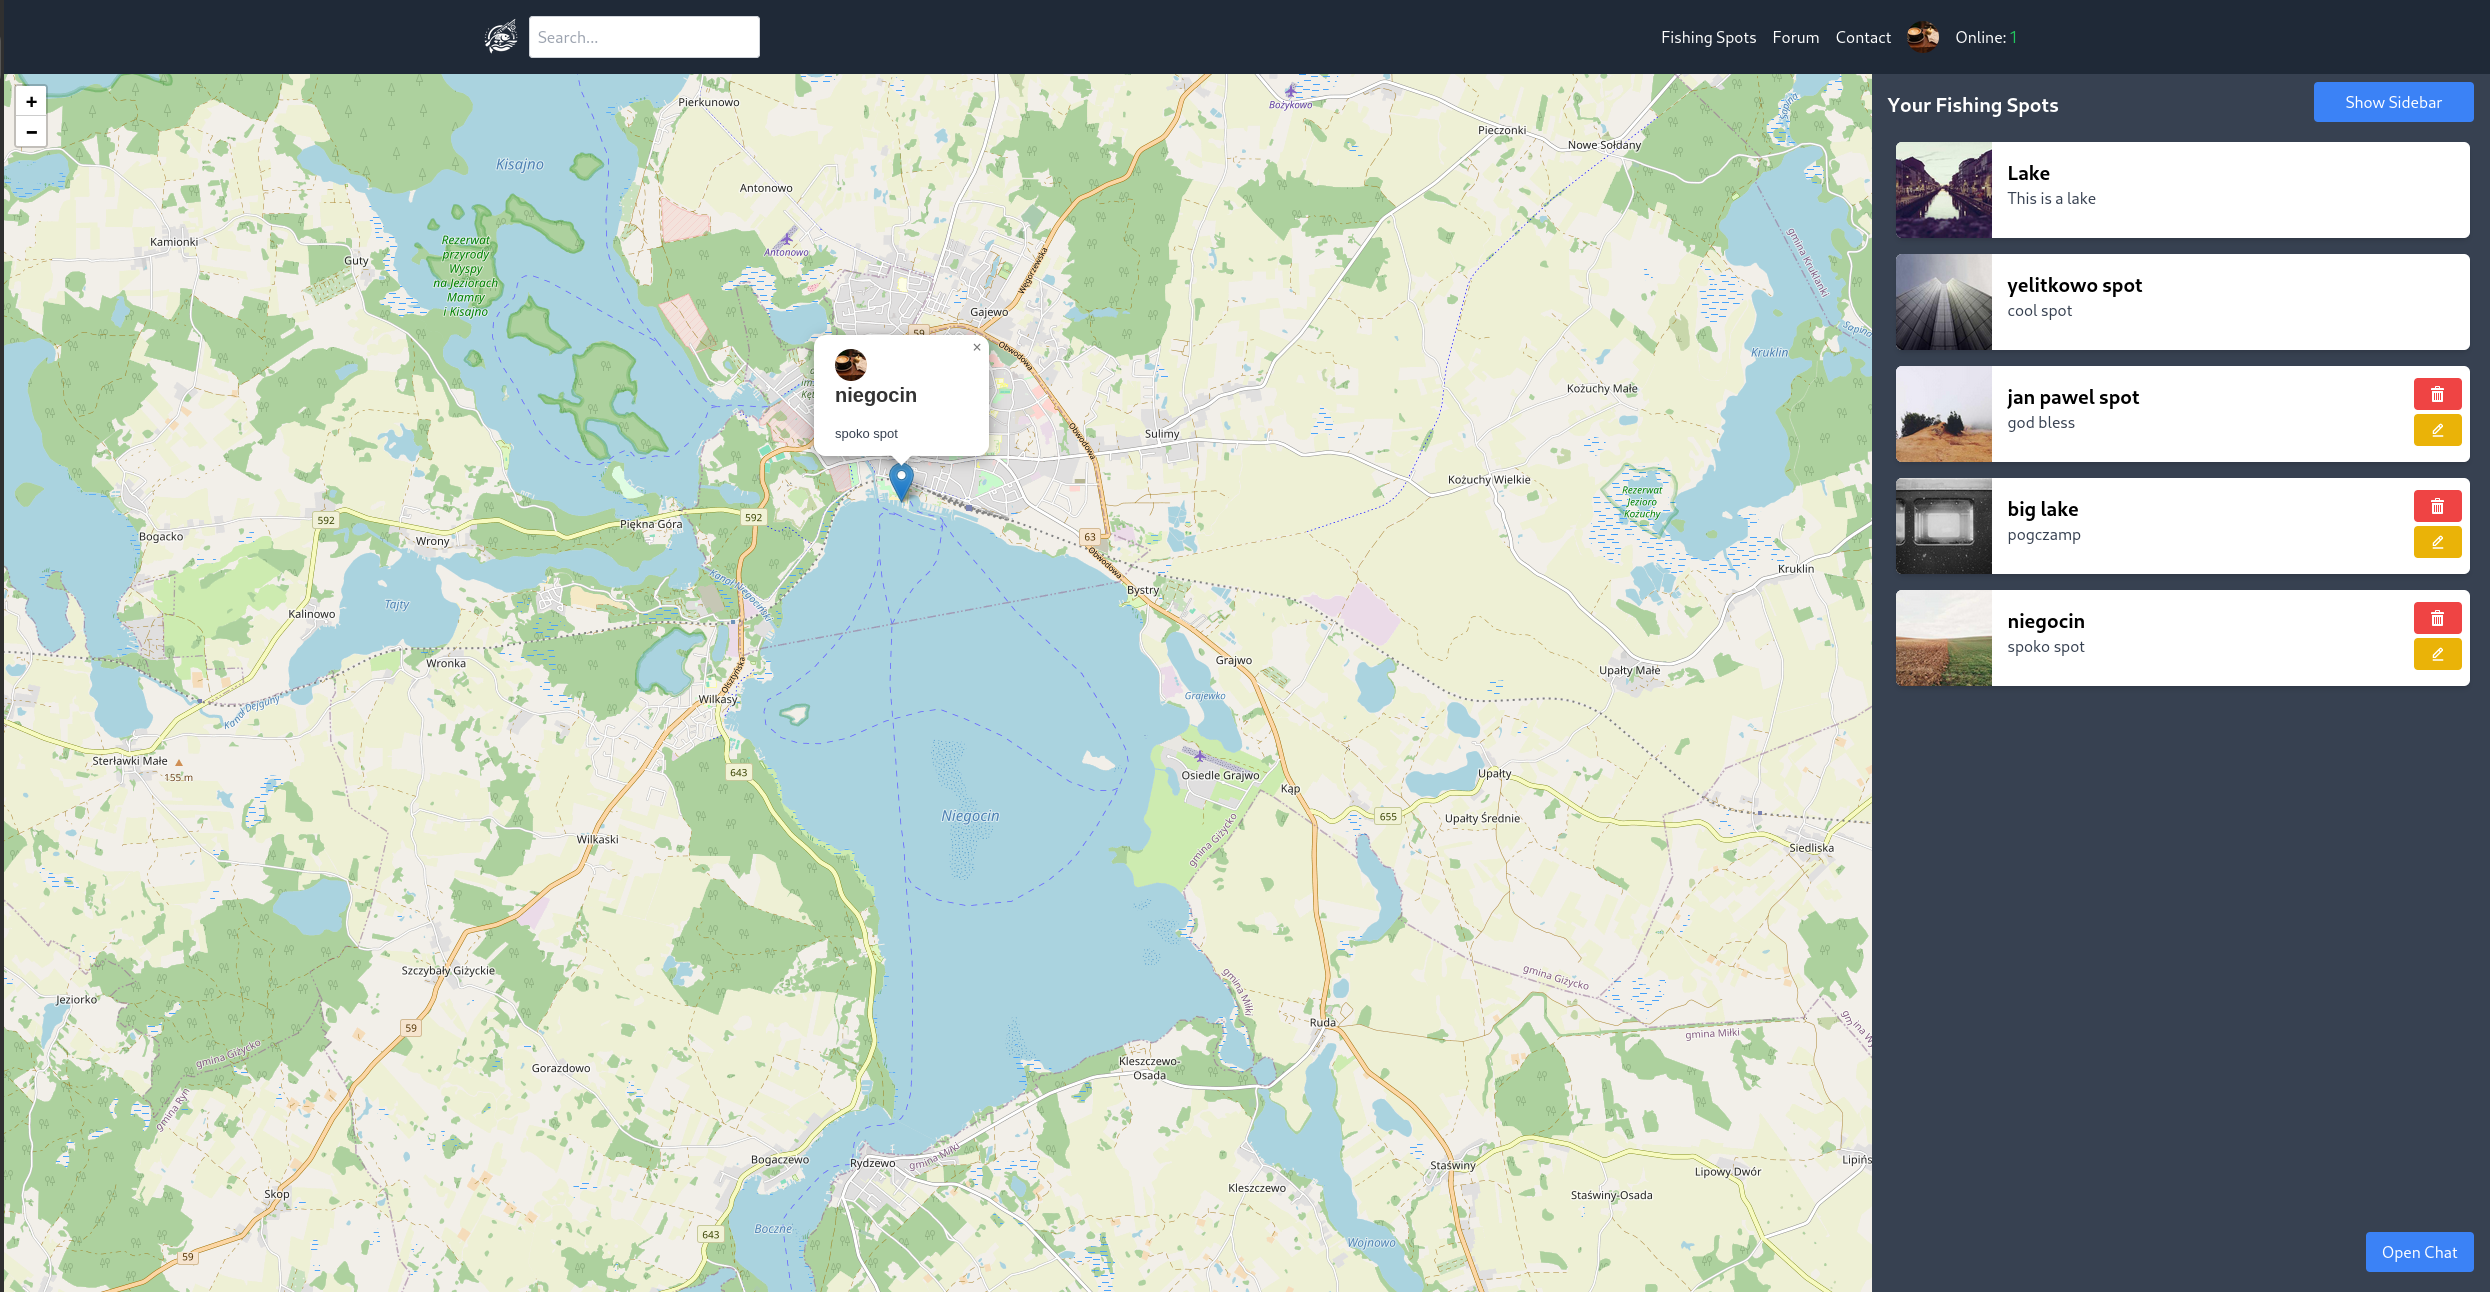
\includegraphics[width=\textwidth]{fishing_spots.png}}
\subsubsection{Przeglądanie profili użytkowników}
\frame{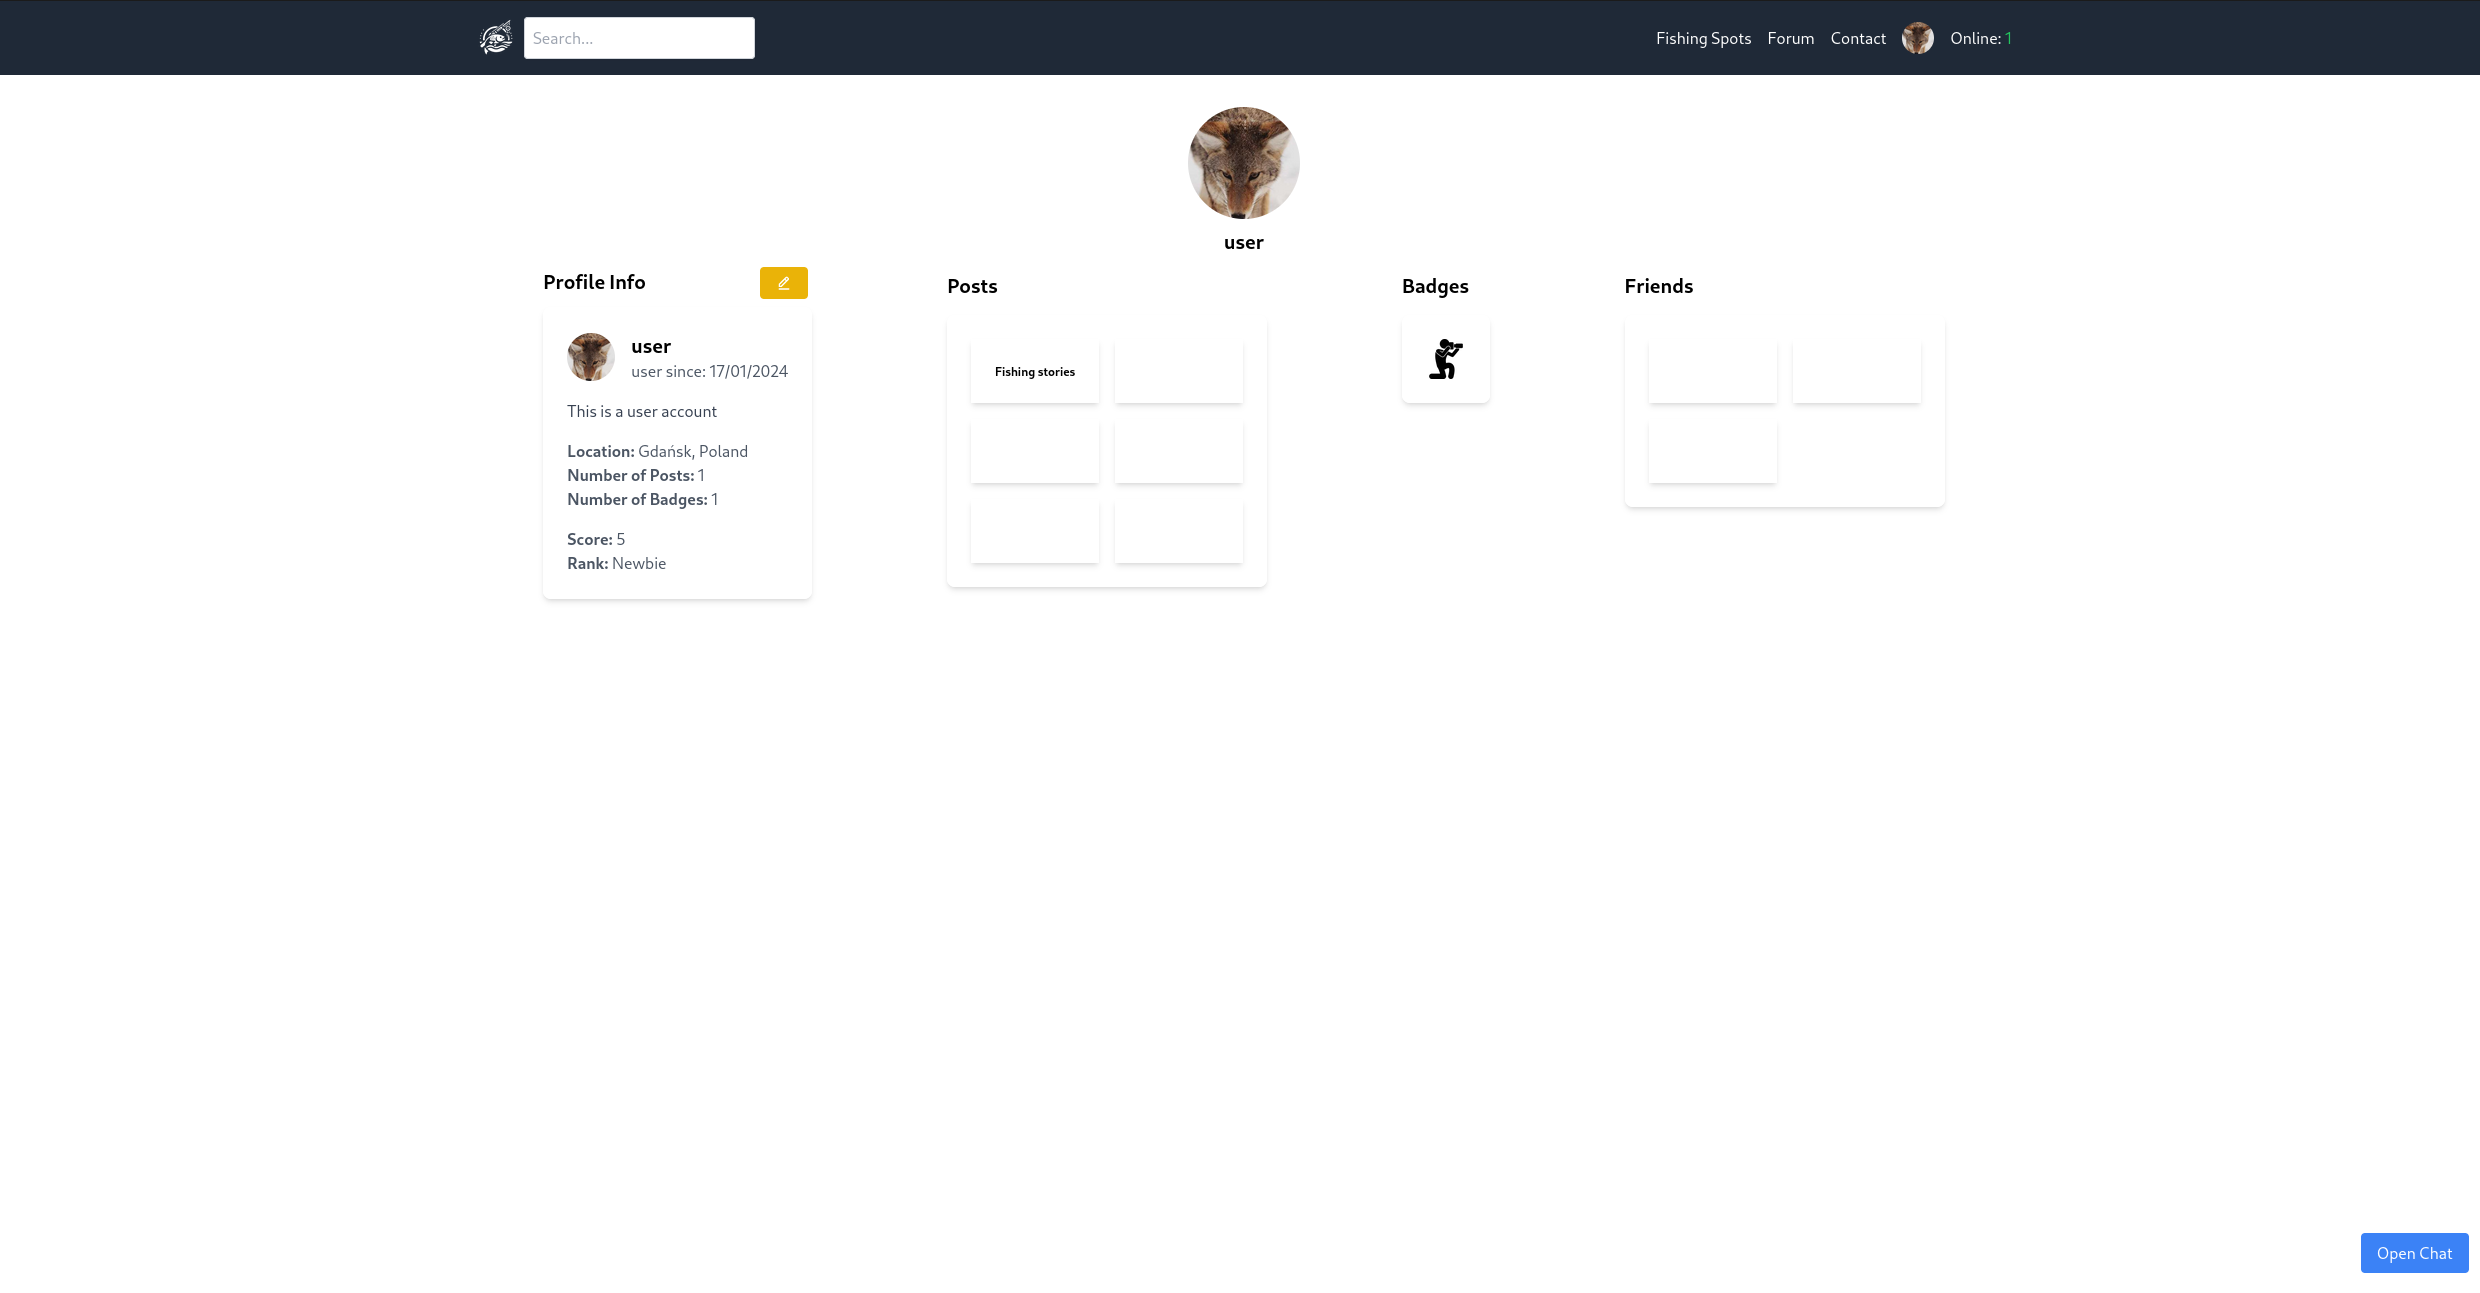
\includegraphics[width=\textwidth]{user_profile.png}}
\subsubsection{Wysyłanie ticketów}
\frame{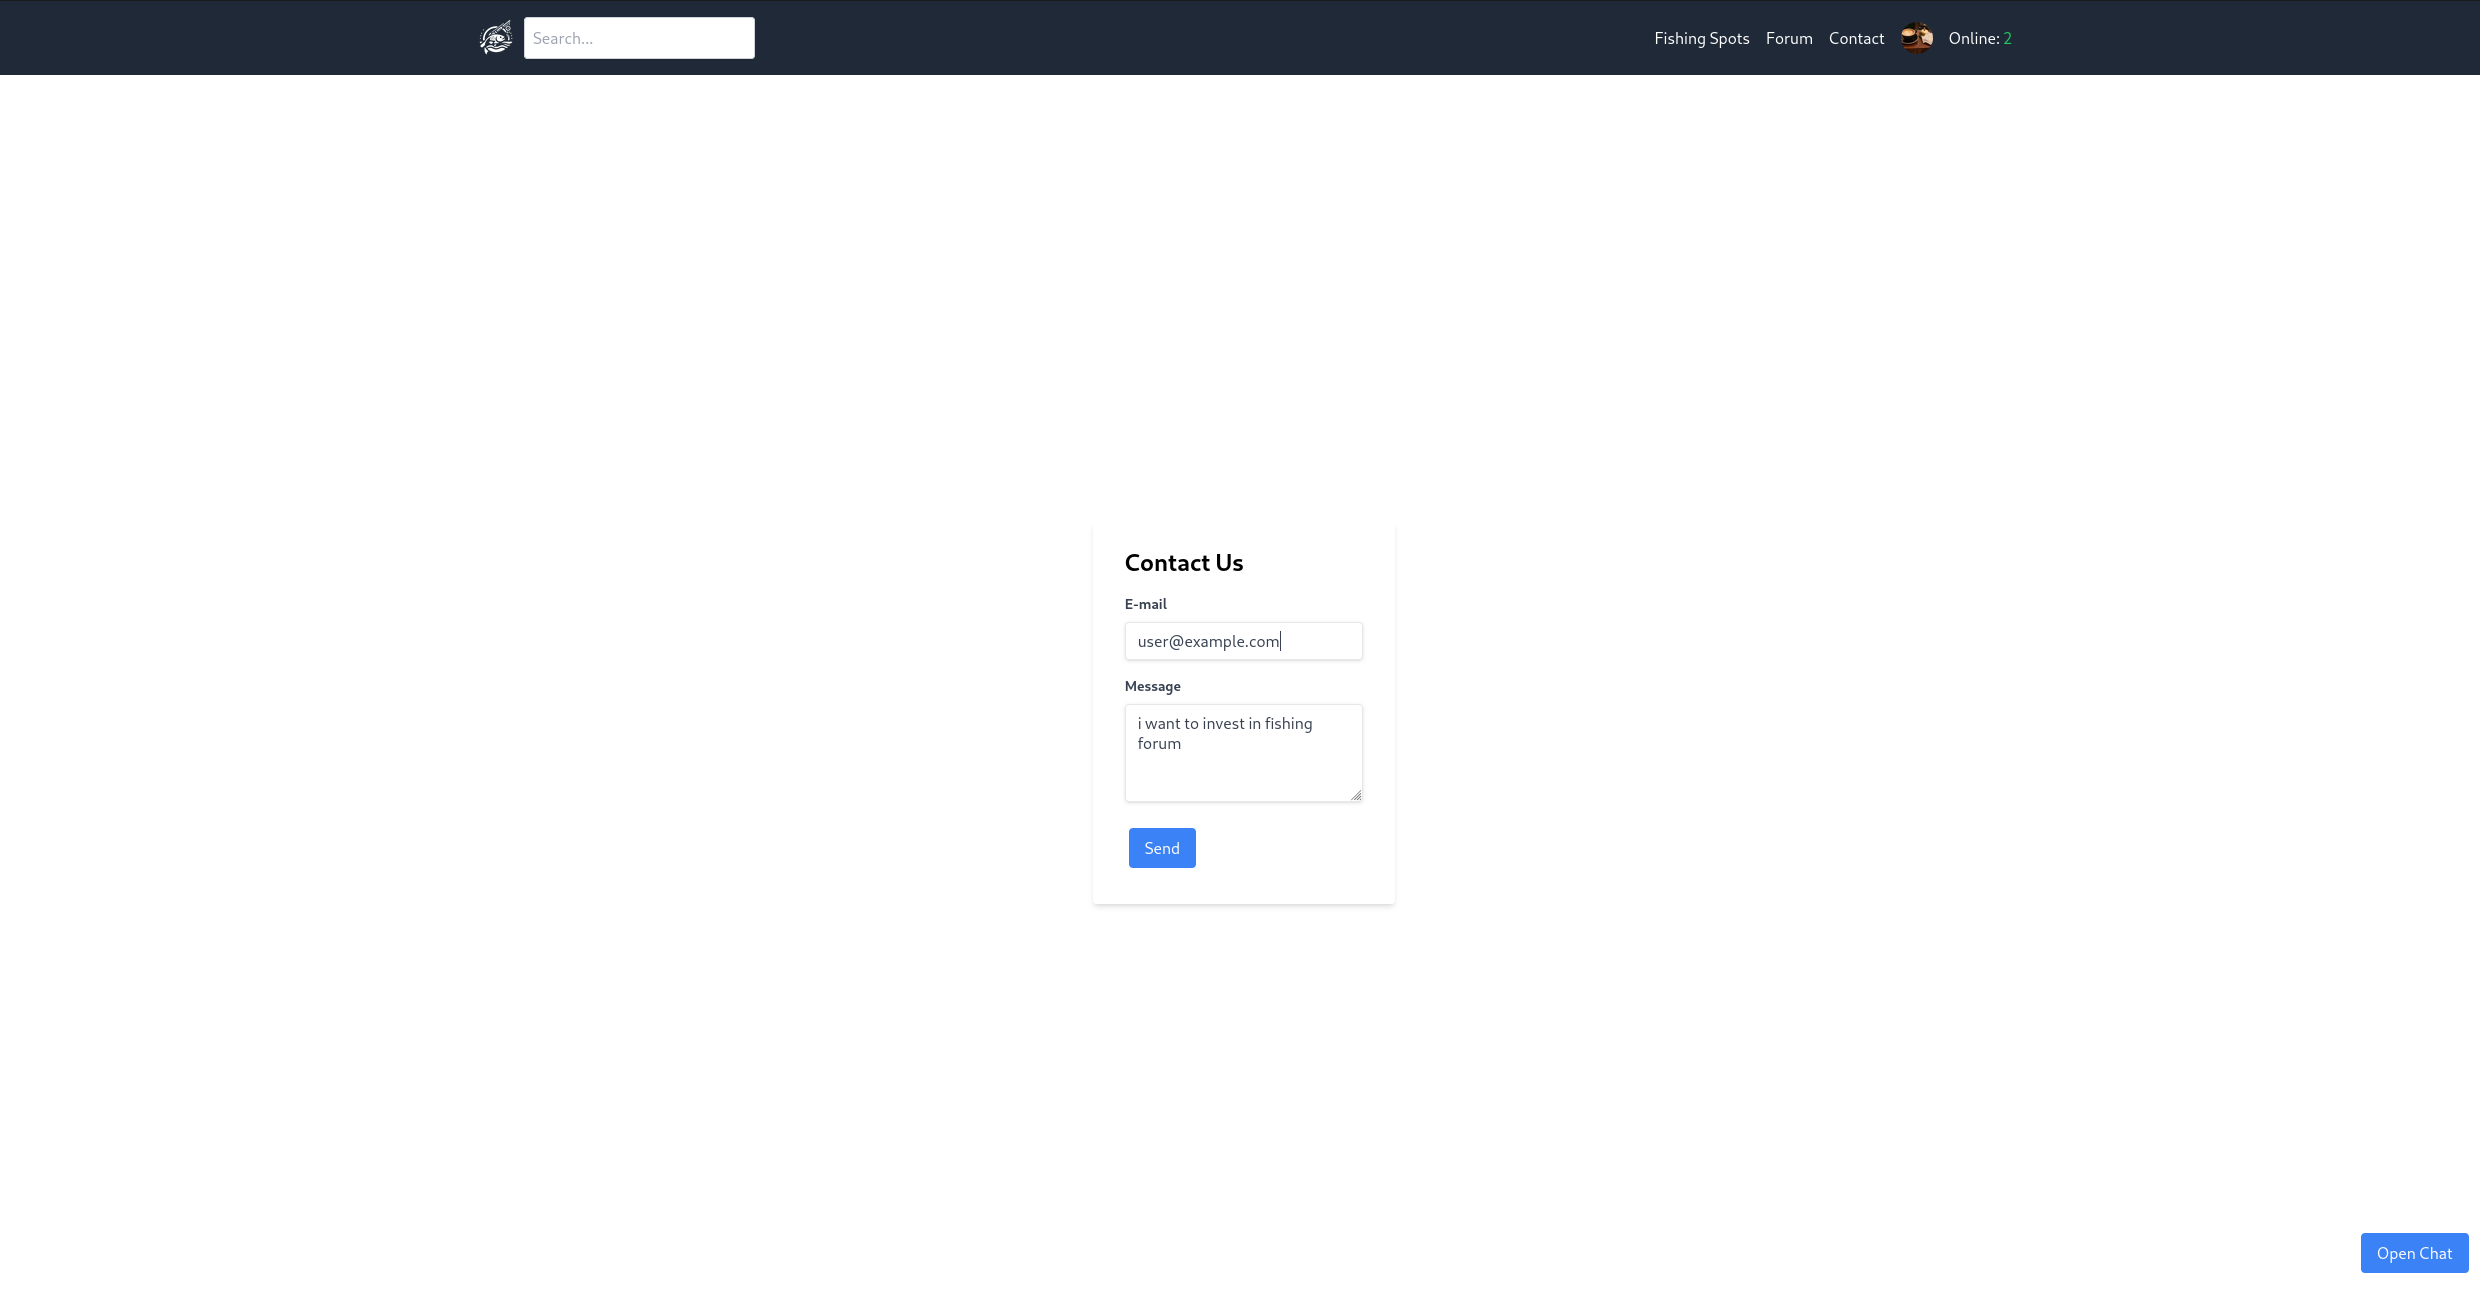
\includegraphics[width=\textwidth]{contact_us.png}}
\subsubsection{Rejestracja i logowanie}
\frame{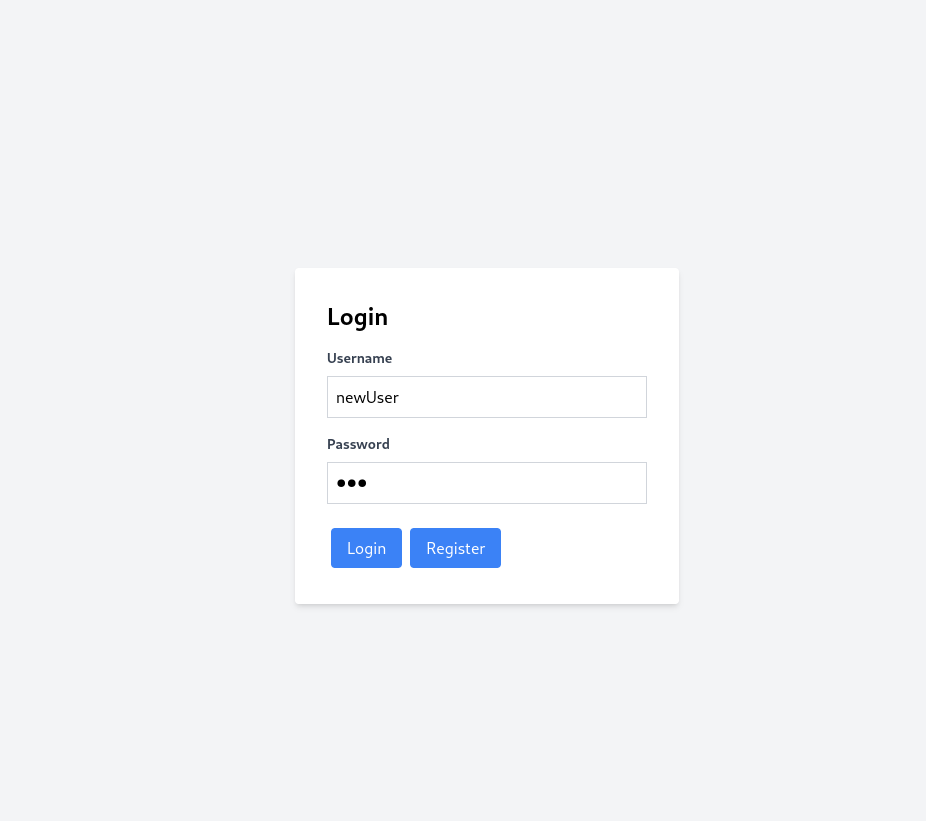
\includegraphics[width=\textwidth]{register_login.png}}
\subsubsection{Wyszukiwanie użytkowników}
\frame{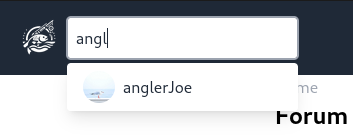
\includegraphics[width=\textwidth]{search_bar.png}}

\subsection{Dla zalogowanych użytkowników}
\subsubsection{Tworzenie postów}
\frame{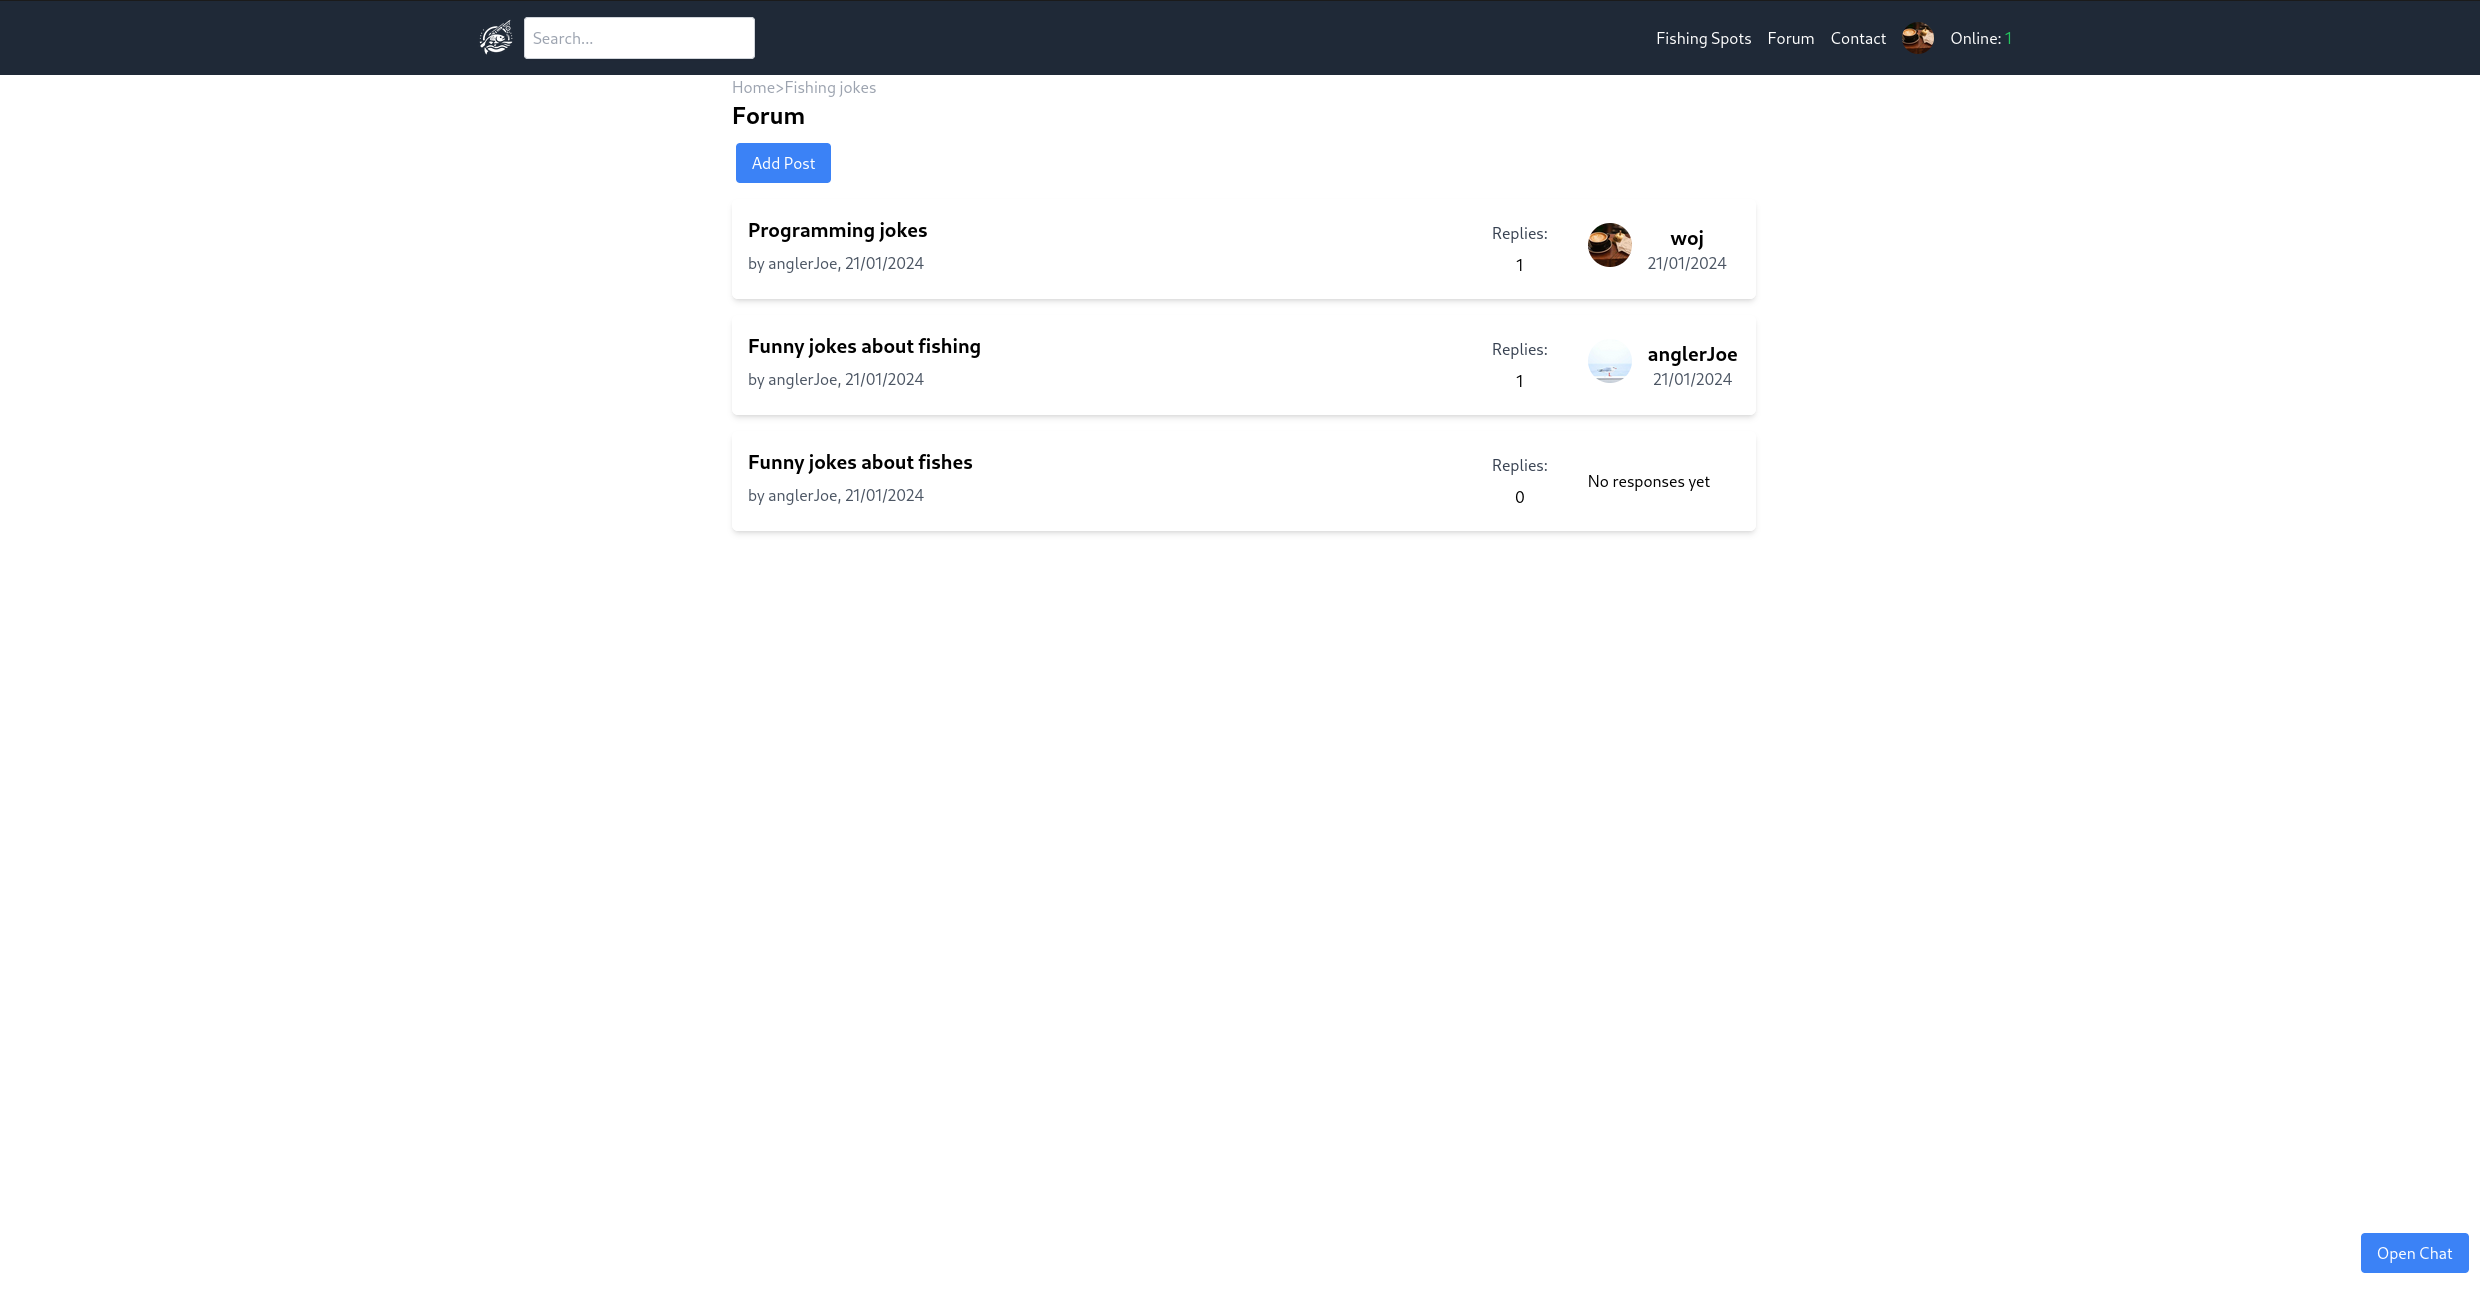
\includegraphics[width=\textwidth]{forum_posts.png}}
\subsubsection{Odpowiadanie na posty}
\frame{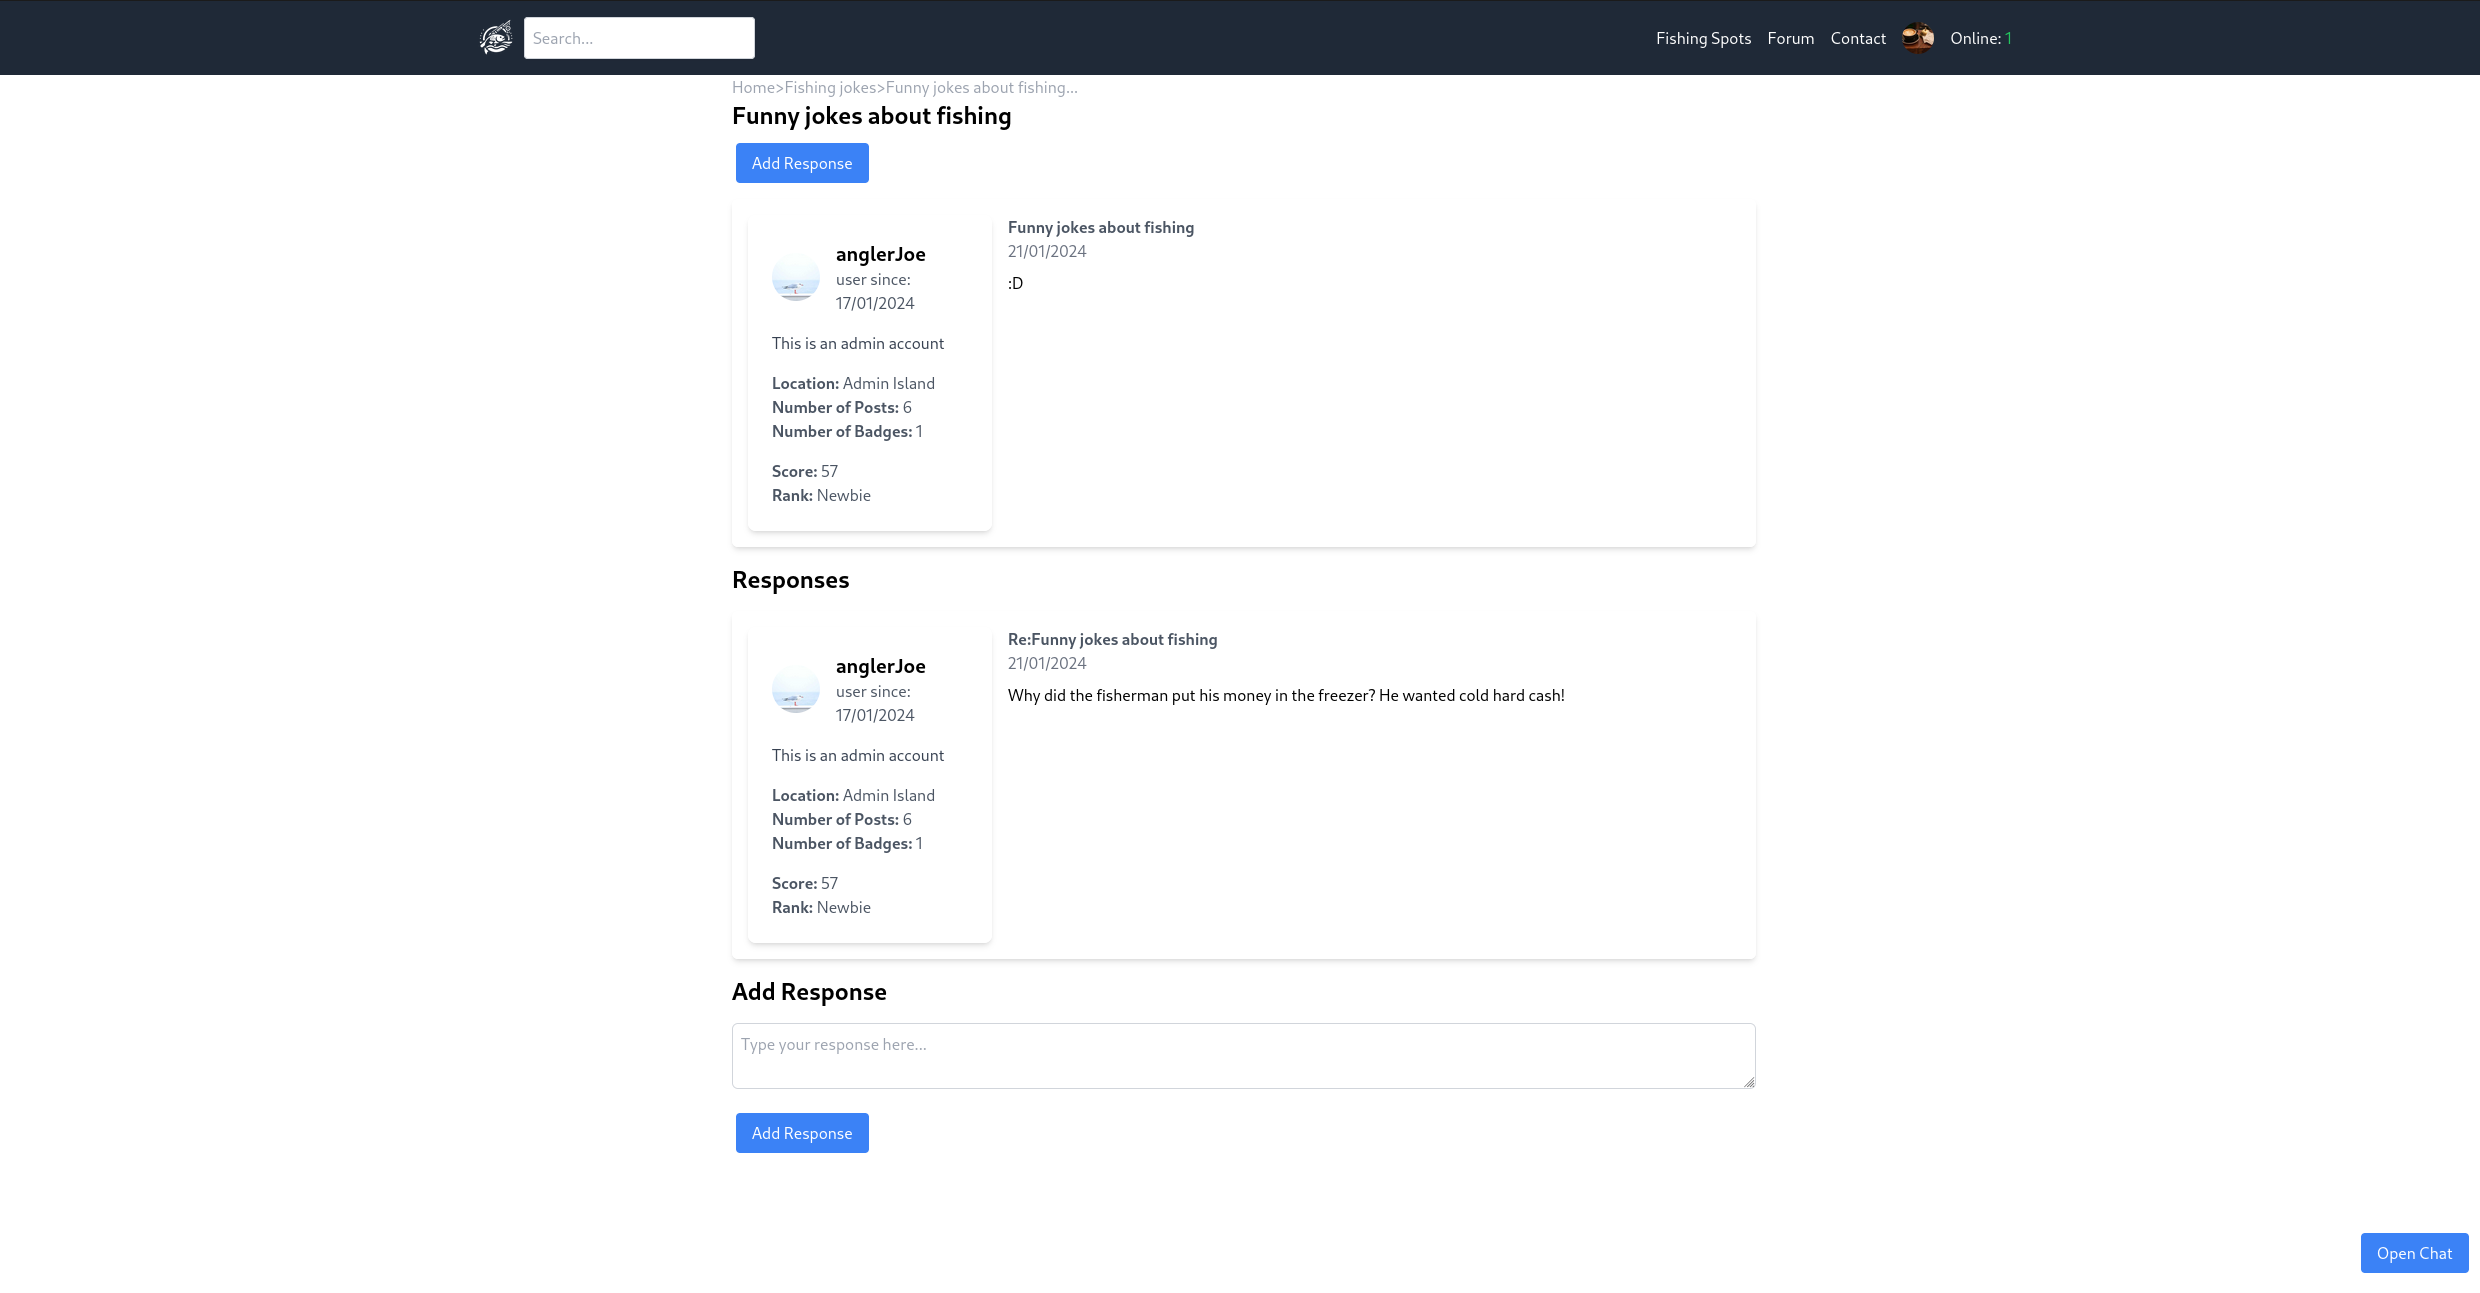
\includegraphics[width=\textwidth]{forum_responses.png}}
\subsubsection{Tworzenie lub edycja miejsc wędkarskich}
\frame{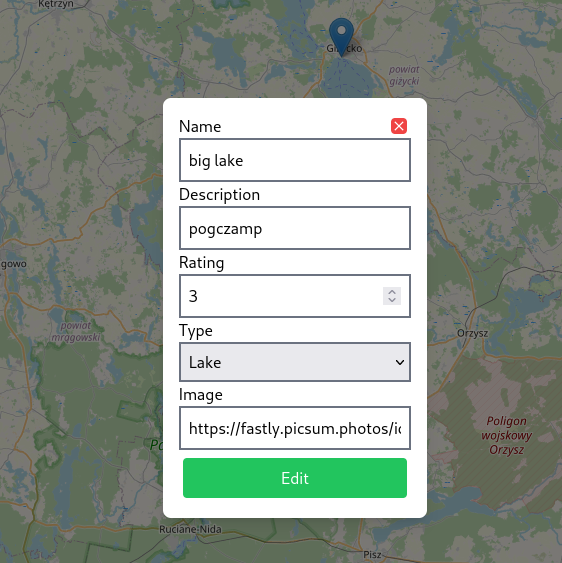
\includegraphics[width=\textwidth]{fishing_spot_edit_add.png}}
\subsubsection{Edycja własnego profilu}
\frame{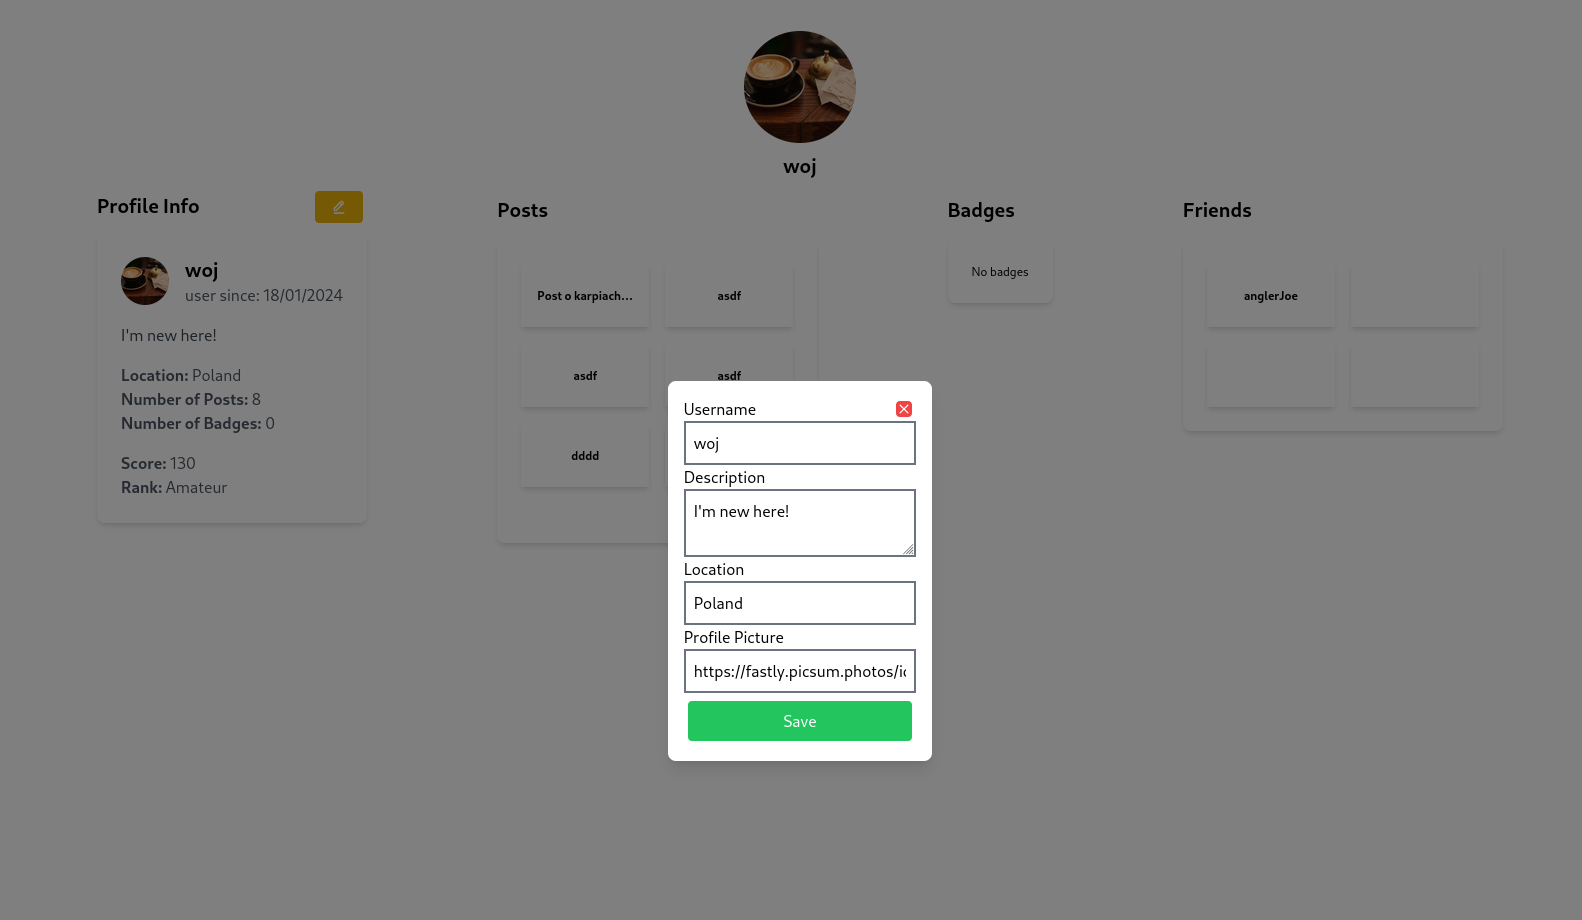
\includegraphics[width=\textwidth]{user_edit.png}}
\subsubsection{Konwersacja z innymi użytkownikami}
\frame{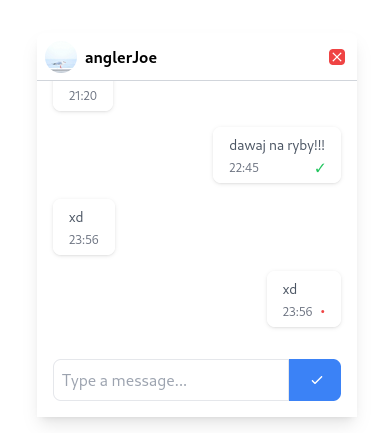
\includegraphics[width=\textwidth]{chat_conversation.png}}
\newpage
\frame{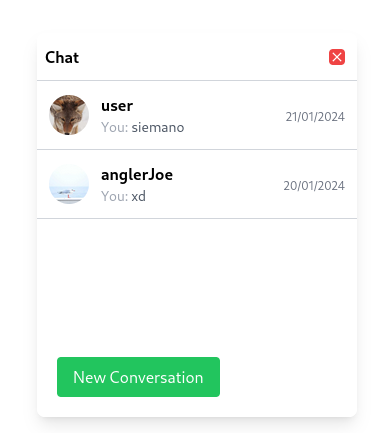
\includegraphics[width=\textwidth]{chat_main.png}}
\frame{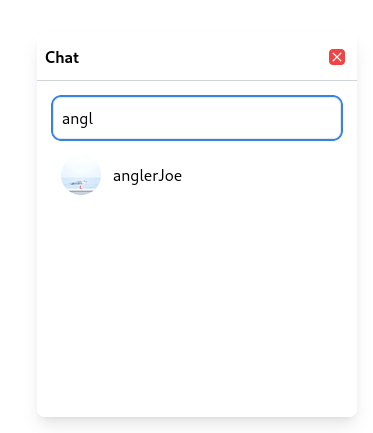
\includegraphics[width=\textwidth]{chat_search.png}}
\frame{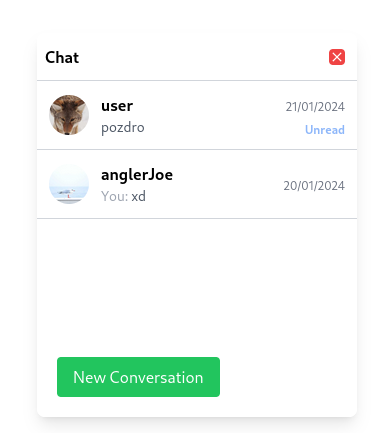
\includegraphics[width=\textwidth]{chat_unread.png}}


\end{document}
